\documentclass{article}
\usepackage[utf8]{inputenc}

\title{\textbf{\textsc{Move the content of one register to another register using 7474IC}}}
\author{\textit{\textbf{R.Radhika}}}
\usepackage{graphicx}
\begin{document}

\maketitle
\section{Abstract}
Design a sequential circuit that shifts its content to another register using 7474IC.
\section{Components}
% Please add the following required packages to your document preamble:
% \usepackage{graphicx}
\begin{table}[ht]
\resizebox{\columnwidth}{!}{%
\begin{tabular}{|l|l|l|}
\hline
\textbf{Component} & \textbf{Value} & \textbf{Quantity} \\ \hline
Bread board & - & 1 \\ \hline
Arduino & Uno & 1 \\ \hline
LED & - & 4 \\ \hline
IC & 7474 & 2 \\ \hline
Jumper Wires & - & 20 \\ \hline
\end{tabular}%
}
\caption{}
\label{Tabel-1}
\end{table}
\section{Procedure}
1.Generate the CLOCK signal using the arduino code
\\
2.Connect the Arduino, LEDs andthe two 7474 ICs according to Table below.
\\
3.Verify the output for the sequence by changing the D1 pin to Vcc and Ground for different clock cycles.
\\

% Please add the following required packages to your document preamble:
% \usepackage{graphicx}
% \usepackage[normalem]{ulem}
% \useunder{\uline}{\ul}{}
\begin{table}[ht]
\resizebox{\columnwidth}{!}{%
\begin{tabular}{|l|ll|l|l|l|lllll|l|l|l|l|l|}
\hline
\textbf{Arduino} & \multicolumn{2}{l|}{{\ul \textit{D13}}} & {\ul \textit{}} & {
\ul \textit{}} & {\ul \textit{}} & \multicolumn{5}{l|}{{\ul \textit{Vcc}}} & {\ul \textit{GND}} &  &  &  &  \\ \hline
\textbf{7474} & \multicolumn{1}{l|}{clk-1} & clk-2 & \begin{tabular}[c]{@{}l@{}}\\
5 - \\ 12\end{tabular} & 9 &  & \multicolumn{1}{l|}{1} & \multicolumn{1}{l|}{4} 
& \multicolumn{1}{l|}{10} & \multicolumn{1}{l|}{13} & 14 & 7 & 5 & 9 &  &  \\ \hline
\textbf{7474} & \multicolumn{1}{l|}{clk-1} & clk-2 &  & 2 & \begin{tabular}[c]{@\\hline
{}l@{}}5 - \\ 12\end{tabular} & \multicolumn{1}{l|}{1} & \multicolumn{1}{l|}{4} 
& \multicolumn{1}{l|}{10} & \multicolumn{1}{l|}{13} & 14 & 7 &  &  & 5 & 9 \\ \hline
\textbf{LED} & \multicolumn{1}{l|}{} &  &  &  &  & \multicolumn{1}{l|}{} & \multicolumn{1}{l|}{} & \multicolumn{1}{l|}{} & \multicolumn{1}{l|}{} &  &  & led1 & 
led2 & led3 & led4 \\ \hline
\end{tabular}%
}
\caption{connections}
\label{tab:my-table}
\end{table}
\section{Truth table}
\\
Give the input sequence 0110 to the register and verify using the truth table.
We need to give the input from LSB to MSB.
\\
\\
-->Try the sequence 1100 using the same circuit and observe the output.
\begin{table}[ht]
\resizebox{\columnwidth}{!}{%
\begin{tabular}{|l|l|l|l|l|}
\hline
\textbf{D1} & \textbf{Q1} & \textbf{Q2} & \textbf{Q3} & \textbf{Q4} \\ \hline
0 & 0 & 0 & 0 & 0 \\ \hline
1 & 1 & 0 & 0 & 0 \\ \hline
1 & 1 & 1 & 0 & 0 \\ \hline
0 & 0 & 1 & 1 & 0 \\ \hline
\textit{\textbf{0}} & \textit{\textbf{0}} & \textit{\textbf{0}} & \textit{\textbf{1}} & \textit{\textbf{1}} \\ \hline
0 & 0 & 0 & 0 & 1 \\ \hline
0 & 0 & 0 & 0 & 0 \\ \hline
\end{tabular}%
}
\caption{}
\label{Truth table}
\end{table}
\section{Code}
Execute the following code using the below provided link
\\
\begin{table}[ht]
\resizebox{\columnwidth}{!}{%
\begin{tabular}{|l|}
\hline
https://github.com/Radhikarkv/fwc_project/assignment.ino\\ \hline
\end{tabular}%
}
\end{table}
\begin{figure}[ht]
\centering
\begin{minipage}[b]{.49\textwidth}
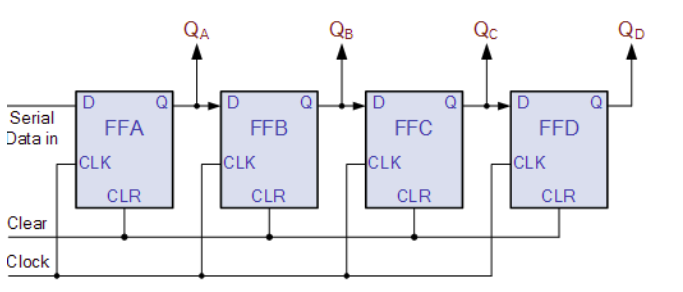
\includegraphics[width=2in]{SIPOregister.png}
\caption{SIPO register}
\label{fig:SIPO}
\end{minipage}
\begin{minipage}[b]{.49\textwidth}
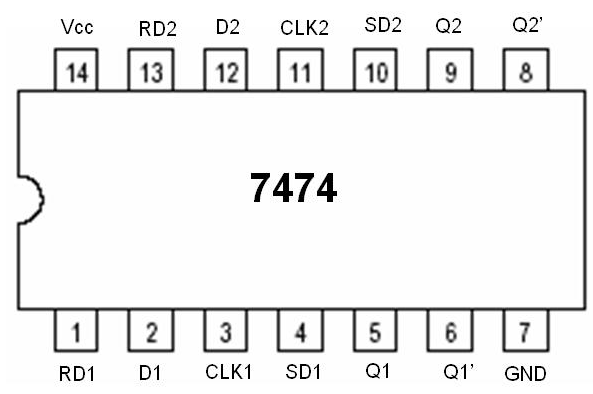
\includegraphics[width=2in]{pindiagram.png}
\caption{pindiagram}
\label{fig:7474}
\end{minipage}
\end{figure}
\end{document}